\chapter{Fusion}
\label{chap:fusion}

This chapter describes the approach taken by the Futhark compiler to
perform loop fusion on SOACs.  Our approach is capable of handling
both \textit{vertical fusion}, where two SOACs are in a
producer-consumer relationship, and \textit{horisontal fusion}, where
two otherwise independent SOACs take the same array as input.  As all
other optimisations in the Futhark compiler, the approach is based on
a syntactic rewriting of abstract syntax trees.

The core of the technique has been previously described in my master's
thesis~\cite{henriksen2014exploiting}.  The current thesis makes three
new contributions:

\begin{enumerate}
\item A simple technique for integrating horisontal fusion in the
  existing framework.  The previously published work did not support
  horisontal fusion at all.
\item Vertical fusion of \lstinline{map} into \lstinline{scan} and
  \lstinline{map} into \lstinline{scatter}.
\item Fusion rules for the streaming SOACs: \lstinline{stream_red},
  \lstinline{stream_map}, and \lstinline{stream_red}.
\end{enumerate}

However, before we can move on to the new contributions, we must
establish the basic fusion algorithm.

The rules by which we combine SOACs through fusion is called the
\textit{fusion algebra}.  The fusion algebra used by the Futhark
compiler has as its central goals to never duplicate computation, and
never reduce available parallelism.  This ensures that the asymptotics
of the program under optimisation are not affected.  Instead, the goal
of fusion is to eliminate the overhead of storing intermediate results
in memory.

Most fusion algorithms in the literature are unable to handle fusion
across \lstinline{zip}/\lstinline{unzip}, and more generally the case
where the output of a producer is used by several consumers.  The
algorithm presented in this chapter is capable of fusing such cases
whenever possible without duplicating computation, as demonstrated on
\cref{fig:fusion-multiple-consumers}.  The linchpin of this capability
is our choice of internal representation, in which arrays of tuples
(and therefore \lstinline{zip}/\lstinline{unzip}) does not occur.

\begin{figure}
\begin{subfigure}[t]{0.4\textwidth}
\begin{lstlisting}
let @b@ = map (+1) a
let c = map (+2) @b@
let d = map (+3) @b@
in map (+) c d
\end{lstlisting}
\caption{Unfused}
\end{subfigure}%
\hspace{.1\textwidth}
\begin{subfigure}[t]{0.4\textwidth}
\begin{lstlisting}
map (\x ->
      let c = x + 2
      let d = x + 3
      in c + d)
    a
\end{lstlisting}
\caption{Fused}
\end{subfigure}%
\caption{Fusing multiple consumers without duplicating computation}
\label{fig:fusion-multiple-consumers}
\end{figure}

This chapter covers two main themes: \Cref{sec:fusionalgebra}
describes informally which producer-consumer we can fuse, as well as
the form of the resulting SOAC.  \Cref{sec:fusion-algorithm} describes
our aggressive fusion algorithm, in particular when a producer result
may be used by multiple consumers, without duplicating computation

\section{Fusion in Futhark}
\label{sec:fusion-in-futhark}

The SOACs we have used so far are a close match to the SOACs of the
source Futhark language.  However, these do not permit a fusion
algebra as rich as we desire.  We extend the existing SOACs, and add a
few more, in order to enable a richer algebra.  Using the previously
shown SOACs, there is not even a way to fuse a composition of
\lstinline{map} and \lstinline{reduce}.

\begin{figure}[hbt]
\begin{tabular}{lcl}
\emph{op} & & \textrm{TySch}(\emph{op}) \\ \hline
  {\lstinline!map!} & : & $\forall d \bar{\alpha}^{(n)}\bar{\beta}^{(m)}. (\alpha_1 \rightarrow \ldots \rightarrow \alpha_n \rightarrow (\bar{\beta}^{(m)}))$ \\
          & & ~~~~~~~~~~~~~~~~~ $\rightarrow [d]\alpha_1 \rightarrow \ldots \rightarrow [d]\alpha_n$ \\
          & & ~~~~~~~~~~~~~~~~~ $\rightarrow ([d]\beta_1,\ldots,[d]\beta_m)$ \\
  {\lstinline!redomap!} & : & $\forall d \bar{\alpha}^{(n)}\bar{\beta}^{(m)}\nseq{\gamma}{l}.$\\
          & & ~~~~~~~~~~~~~~ $(\alpha_1 \rightarrow \ldots \rightarrow \alpha_n \rightarrow \alpha_1 \rightarrow \ldots \rightarrow \alpha_n \rightarrow (\bar{\alpha}^{(n)}))$\\
          & & ~~~~~~~~~~ $\rightarrow (\alpha_1 \rightarrow \ldots \rightarrow \alpha_n \rightarrow \beta_1 \rightarrow \ldots \rightarrow \beta_m \rightarrow (\bar{\alpha}^{(n)}, \bar{\gamma}^{(l)}))$ \\
          & & ~~~~~~~~~~ $\rightarrow (\alpha_1, \ldots, \alpha_n)$\\
          & & ~~~~~~~~~~ $\rightarrow [d]\beta_1 \rightarrow \ldots \rightarrow [d]\beta_n$\\
          & & ~~~~~~~~~~ $\rightarrow (\alpha_1,\ldots,\alpha_n,[d]\gamma_{1},\ldots,[d]\gamma_{l})$ \\
  {\lstinline!scanomap!} & : & $\forall d \bar{\alpha}^{(n)}\bar{\beta}^{(m)}\nseq{\gamma}{l}.$\\
          & & ~~~~~~~~~~~~~~ $(\alpha_1 \rightarrow \ldots \rightarrow \alpha_n \rightarrow \alpha_1 \rightarrow \ldots \rightarrow \alpha_n \rightarrow (\bar{\alpha}^{(n)}))$\\
          & & ~~~~~~~~~~ $\rightarrow (\alpha_1 \rightarrow \ldots \rightarrow \alpha_n \rightarrow \beta_1 \rightarrow \ldots \rightarrow \beta_m \rightarrow (\bar{\alpha}^{(n)}, \bar{\gamma}^{(l)}))$ \\
          & & ~~~~~~~~~~ $\rightarrow (\alpha_1, \ldots, \alpha_n)$\\
          & & ~~~~~~~~~~ $\rightarrow [d]\beta_1 \rightarrow \ldots \rightarrow [d]\beta_n$\\
          & & ~~~~~~~~~~ $\rightarrow ([d]\alpha_1,\ldots,[d]\alpha_n,[d]\gamma_{1},\ldots,[d]\gamma_{l})$ \\
  {\lstinline!scatter!} & : & $\forall d \nseq{x}{m} \bar{\alpha}^{(n)}\bar{\beta}^{(m)}.$\\
          & & ~~~~~~~~~~~~~~ $(\alpha_1 \rightarrow \ldots \rightarrow \alpha_n \rightarrow (\texttt{i32}, \beta_{1}, \ldots, \texttt{i32}, \beta_{m}))$\\
          & & ~~~~~~~~~~ $\rightarrow [x_{1}]\beta_1 \rightarrow \ldots \rightarrow [x_{m}]\beta_m$\\
          & & ~~~~~~~~~~ $\rightarrow [d]\alpha_1 \rightarrow \ldots \rightarrow [d]\alpha_n$\\
          & & ~~~~~~~~~~ $\rightarrow ([x_{1}]\beta_1, \ldots, [x_{m}]\beta_n)$\\
  {\lstinline!stream_par!} & : & $\forall d x \bar{\alpha}^{(n)}\bar{\beta}^{(m)}\nseq{\gamma}{l}.$\\
          & & ~~~~~~~~~~~~~~ $(\alpha_1 \rightarrow \ldots \rightarrow \alpha_n \rightarrow \alpha_1 \rightarrow \ldots \rightarrow \alpha_n \rightarrow (\bar{\alpha}^{(n)}))$\\
          & & ~~~~~~~~~~ $\rightarrow ((x: \texttt{i32}) \rightarrow [x]\alpha_1 \rightarrow \ldots \rightarrow [x]\alpha_n \rightarrow (\bar{\beta}^{(m)}, \nseq{[x]\gamma}{l}))$ \\
          & & ~~~~~~~~~~ $\rightarrow [d]\beta_1 \rightarrow \ldots \rightarrow [d]\beta_n$\\
          & & ~~~~~~~~~~ $\rightarrow (\alpha_1,\ldots,\alpha_n,[d]\gamma_{1},\ldots,[d]\gamma_{l})$ \\
  {\lstinline!stream_seq!} & : & $\forall d x \bar{\alpha}^{(n)}\bar{\beta}^{(m)}\nseq{\gamma}{l}.$\\
          & & ~~~~~~~~~~ $\rightarrow ((x: \texttt{i32})$ \\
          & & ~~~~~~~~~~~~~~~ $\rightarrow \alpha_1 \rightarrow \ldots \rightarrow \alpha_n$ \\
          & & ~~~~~~~~~~~~~~~ $\rightarrow [x]\alpha_1 \rightarrow \ldots \rightarrow [x]\alpha_n$ \\
          & & ~~~~~~~~~~~~~~~ $\rightarrow (\bar{\beta}^{(m)}, \nseq{[x]\gamma}{l}))$ \\
          & & ~~~~~~~~~~ $\rightarrow (\alpha_1, \ldots, \alpha_n)$\\
          & & ~~~~~~~~~~ $\rightarrow [d]\beta_1 \rightarrow \ldots \rightarrow [d]\beta_n$\\
          & & ~~~~~~~~~~ $\rightarrow (\alpha_1,\ldots,\alpha_n)$ \\

\end{tabular}
\caption{Extended SOACs used for fusion and later stages of the compiler.}
\label{fig:soacType}
\end{figure}

We will assume that all instances of \texttt{replicate(n,x)} have been
rewritten as \texttt{map(fn~t~(int~i)~=>~x,~iota(n))}\footnote{In the
  actual implementation, we convert these back into \texttt{replicate}
  expressions if they are not fused, but for clarity the bookkeeping
  necessary is elided in this presentation.}.

\Cref{fig:producers-consumers} lists which Futhark SOACs are producers,
which are consumers, and which are both.  In particular, note that
even if we have a \texttt{reduce}-expression returning an array, this
does not mean that the \texttt{reduce}-expression is a producer -
because, in our algebra, it cannot be fused into another SOAC
expression.  The reason is that the output of the reduction is only
fully known after the final input array element has been processed.
Consider the following program:

\begin{lstlisting}
let b = reduce(fn [int] ([int] acc, int x) =>
                 map(op + (x), acc),
               iota(10), a) in
map(f, b)
\end{lstlisting}

The contents of the array \texttt{b} is not determined until the very
last element of \texttt{a} has been processed, and thus fusion with
the \texttt{map}-expression cannot take place.  While it is possible
to use \texttt{reduce} in a way that could theoretically be fused with
a consumer (for example by using it to simulate \texttt{map}), the
analysis necessary to determine whether a given reduction is fusible
would be quite onerous, and likely not useful in any but contrived
examples, such as the above-mentioned simulation of \texttt{map}.

In this way, \texttt{reduce} differs from \texttt{map}, in which each
element of the output is calculated from one element of the input ---
a classic case of data-parallelism.

Even if we have a producer-consumer-pair, not all such pairs
\textit{can} be fused, and not all are \textit{desirable} to fuse.
For instance, \texttt{filter}-\texttt{map} fusion is not possible,
although \texttt{filter}-\texttt{reduce} is.  The reason is that, with
the former, the size of the \texttt{map}-output is the same as the
size of its input, yet the size of the output of \texttt{filter}
cannot be known in advance, which precludes an efficient fused form.

\subsection{Fusion algebra}
\label{sec:fusionalgebra}

In this section, we will give an informal introduction to which SOACs
can be fused, as well as the form of the result.  In order to preserve
clarity, we will not go into great detail until
\cref{sec:fusion-rules}.

\subsubsection{\texttt{map-map} fusion}

The quintessential example of fusion is composing two consecutive
\texttt{map} operations into a single \texttt{map}, as follows:

\begin{lstlisting}
let \{x1, x2\} = mapT(f, a1)
in  mapT(g, x1, y)
    \emphh{\mymath{\Downarrow}}
mapT(fn \mymath{\beta} (\mymath{\alpha\myindx{1}} a1\mymath{\myindx{i}}, \mymath{\alpha\myindx{2}} y\mymath{\myindx{i}}) =>
      let \{x1\mymath{\myindx{i}}, x2\mymath{\myindx{i}}\} = f(a1\mymath{\myindx{i}})
      in  g(x1\mymath{\myindx{i}}, y\mymath{\myindx{i}})
    , a1, y )
\end{lstlisting}

\subsubsection{\texttt{replicate} fusion}

\texttt{replicate} is an interesting case.  We wish to always be able
to fuse replicate into a consumer, like this:

\begin{lstlisting}
let x = replicate(N,a) in
mapT(f, x) in
    \emphh{\mymath{\Downarrow}}
mapT(fn \mymath{\beta\myindx{1}} (int i) =>
       f(a), b)
\end{lstlisting}

And indeed, this can be done through ordinary \texttt{map}-fusion if
\texttt{replicate(N,a)} is first rewritten to \texttt{map} as
described in \cref{sec:fusion-in-l0}.

\subsubsection{\texttt{map-reduce} and \texttt{map-scan} fusion}

The result of \texttt{map}-\texttt{reduce}-fusion is normally
\texttt{redomap}.

\begin{lstlisting}
let \{x1, x2\} = mapT(f, a1)
in  reduceT(\mymath{\oplus},e\mymath{\myindx{1}},e\mymath{\myindx{2}}, x1,y)
    \emphh{\mymath{\Downarrow}}
redomapT(\mymath{\oplus}
, fn (\mymath{\beta\myindx{1}},\mymath{\beta\myindx{2}}) ( \mymath{\beta\myindx{1}} e\mymath{\myindx{1}}, \mymath{\beta\myindx{2}} e\mymath{\myindx{2}}
             , \mymath{\alpha\myindx{1}} a1\mymath{\myindx{i}},\mymath{\alpha\myindx{2}} y\mymath{\myindx{i}})
   => let \{x1\mymath{\myindx{i}}, x2\mymath{\myindx{i}}\} = f(a1\mymath{\myindx{i}})
      in  \mymath{\oplus}(e\mymath{\myindx{1}},e\mymath{\myindx{2}},x1\mymath{\myindx{i}},y\mymath{\myindx{i}})
, (e\mymath{\myindx{1}}, e\mymath{\myindx{2}}), a1, y )
\end{lstlisting}

In general, we cannot fuse \texttt{map} and \texttt{reduce} to another
\texttt{reduce}, as the accumulator type of a reduction must match the
element type of the input array. Adding the input of the \texttt{map}
to the input of the \texttt{reduce} may violate this requirement, as
demonstrated on \cref{fig:map-reduce-error}.

\begin{figure}
\begin{center}
\begin{lstlisting}
let \{c\} = mapT(fn \{int\} (int x, int y) => \{x+y\},
                 a, b) in
reduceT(op +, \{0\}, c)
  \(\emphh{\Downarrow}\)
reduceT(fn int (int acc, int x, int y) => acc + x + y,
        \{0\}, a, b) \emp{// Type error, as accumulator}
                   \emp{// type must match array input type}
\end{lstlisting}
\end{center}

\caption{Cannot fuse to \texttt{reduce} (but \texttt{redomap} would be valid)}
\label{fig:map-reduce-error}
\end{figure}

The solution is to first rewrite \texttt{reduceT($\oplus$,$x$,$a$)} to
\texttt{redomapT($\oplus$,$\oplus$,$x$,$a$)}, since we can always fuse
\texttt{map} with \texttt{redomap}:

\begin{lstlisting}
let \{x1, x2\} = mapT(f, a1)
in  redomapT(\mymath{\oplus}, g, e, x1, y)
    \emphh{\mymath{\Downarrow}}
redomapT(\mymath{\oplus}
, fn \mymath{\beta} (\mymath{\beta} e, \mymath{\alpha\myindx{1}} a1\mymath{\myindx{i}}, \mymath{\alpha\myindx{2}} y\mymath{\myindx{i}})
   => let \{x1\mymath{\myindx{i}}, x2\mymath{\myindx{i}}\} = f(a1\mymath{\myindx{i}})
      in  g(e, x1\mymath{\myindx{i}}, y\mymath{\myindx{i}})
, e, a1, y )
\end{lstlisting}

However, there are a few rare cases where we can fuse \texttt{map} and
\texttt{reduce} to \texttt{reduce}.  This only happens when the
\textit{input} to the map has the same count and types as the outputs
of the \texttt{map} that are being used as input to the
\texttt{reduce}.

\begin{lstlisting}
let \{x\cindx{1}, x\cindx{2}\} = mapT(f, a\cindx{1}, a\cindx{2})
in  reduceT(\mymath{\oplus},\{e\cindx{1}, e\cindx{2}, e\cindx{3}\}, x\cindx{1}, x\cindx{2}, y)
    \emphh{\mymath{\Downarrow}}
reduceT(fn (\(\alpha\myindx{1}\),\(\alpha\myindx{2}\)) ( \(\alpha\myindx{1}\) x\cindx{1}, \(\alpha\myindx{2}\) x\cindx{2}, \(\alpha\myindx{3}\) x\cindx{3},
            \(\alpha\myindx{1}\) ai\cindx{1}, \(\alpha\myindx{2}\) ai\cindx{2}, \(\alpha\myindx{3}\) ye) =>
          let \{x\cindx{1}, x\cindx{2}\} = f(ae\cindx{1}, ae\cindx{2})
          in  \mymath{\oplus}(x\cindx{1}, x\cindx{2}, x\cindx{3}, x\cindx{1}, x\cindx{2}, ye)
        , \{e\cindx{1}, e\cindx{2}, e\cindx{3}\}, a\cindx{1}, a\cindx{2}, y)
\end{lstlisting}

In fact, under these circumstances we can also fuse \texttt{map} with
\texttt{scan}:

\begin{lstlisting}
let \{x\cindx{1}, x\cindx{2}\} = mapT(f, a\cindx{1}, a\cindx{2})
in  scanT(\mymath{\oplus},\{e\cindx{1}, e\cindx{2}, e\cindx{3}\}, x\cindx{1}, x\cindx{2}, y)
    \emphh{\mymath{\Downarrow}}
scanT(fn (\(\alpha\myindx{1}\),\(\alpha\myindx{2}\)) ( \(\alpha\myindx{1}\) x\cindx{1}, \(\alpha\myindx{2}\) x\cindx{2}, \(\alpha\myindx{3}\) x\cindx{3},
          \(\alpha\myindx{1}\) ai\cindx{1}, \(\alpha\myindx{2}\) ai\cindx{2}, \(\alpha\myindx{3}\) ye) =>
        let \{x\cindx{1}, x\cindx{2}\} = f(ae\cindx{1}, ae\cindx{2})
        in  \mymath{\oplus}(x\cindx{1}, x\cindx{2}, x\cindx{3}, x\cindx{1}, x\cindx{2}, ye),
      \{e\cindx{1}, e\cindx{2}, e\cindx{3}\}, a\cindx{1}, a\cindx{2}, y)
\end{lstlisting}

It should be clear that the composed function is still associative, as
required by \texttt{scan} and \texttt{reduce}.

\subsubsection{\texttt{filter-filter} fusion}

Fusing \texttt{filter-filter} is quite simple - it's a new
\texttt{filter} SOAC where both of the filter functions must return
true for each element.  However, we can only perform the fusion if the
input set of the consumer is a subset of the output set of the
producer.  Put another way, the consumer must accept input from no
other source than the producer involved in the fusion.\footnote{The
  implementation in the Futhark compiler is currently even more
  restrictive, in that the input set of the consumer must match the
  output set of the producer \textit{exactly}.  Fixing this oversight
  is left as an exercise for the author.}

\begin{lstlisting}
let \{x\cindx{1},x\cindx{2}\}=filterT(c\cindx{1},a\cindx{1},a\cindx{2}) in
let \{y\} = filterT(c\cindx{2}, x\cindx{1}) in
...
    \emphh{\mymath{\Downarrow}}
let \{y, _\} = filterT(fn bool (\(\alpha\myindx{1}\) ai\cindx{1},\(\alpha\myindx{2}\) ai\cindx{2}) =>
                       if   c\cindx{1}(ai\cindx{1}, ai\cindx{2})
                       then c\cindx{2}(ai\cindx{1})
                       else False,
                     a\cindx{1}, a\cindx{2} ) in
...
\end{lstlisting}

As a bit of a technical curiosity, we are forced to use an
\texttt{if}-expression, as the \texttt{\&\&} operator in Futhark is not
short-circuiting.

\subsubsection{\texttt{filter-reduce} fusion}

We can fuse \texttt{filter} with \texttt{reduce} and obtain
\texttt{reduce} \textit{only} in the case where the input set of the
\texttt{reduce} is equal to the output set of the \texttt{filter}.

\begin{lstlisting}
let \{x\} = filterT(c, a) in
reduceT(\mymath{\oplus}, e, x)
    \emphh{\mymath{\Downarrow}}
reduceT(fn \(\beta\) (\(\beta\) e, \(\beta\) ai) =>
          if c(ai) then \(\oplus\)(e,ai) else e,
        \{e\}, a)
\end{lstlisting}

We can fuse \texttt{filter} with \texttt{reduce} and obtain
\texttt{redomapT} if the input set of the \texttt{reduce} is included
in the output set of the \texttt{filter}.

\begin{lstlisting}
let \{x1,x2\} = filterT(c, a\cindx{1}, a\cindx{2})
in  reduceT(\(\oplus\), \{e\}, x\cindx{1})
    \emphh{\mymath{\Downarrow}}
redomapT(\(\oplus\),
         fn \(\beta\) (\(\beta\) e, \(\alpha\myindx{1}\) ai\cindx{1}, \(\alpha\myindx{2}\) ai\cindx{2}) =>
           if c(ai\cindx{1}, ai\cindx{2})
           then \(\oplus\)(e, ai\cindx{1})
           else e,
         \{e\}, a\cindx{1}, a\cindx{2})
\end{lstlisting}

\subsubsection{\texttt{filter-redomap} fusion}

Similarly, we can fuse \texttt{filter} with \texttt{redomapT} and
obtain \texttt{redomapT} if the input set of the \texttt{reduce} is
included in the output set of the \texttt{filter}.

\begin{lstlisting}
let \{x\cindx{1},x\cindx{2}\}=filterT(c, a\cindx{1}, a\cindx{2})
in  redomapT(\(\oplus\), g, \{e\}, x\cindx{1})
    \emphh{\(\Downarrow\)}
redomapT(\(\oplus\),
         fn \(\beta\) (\(\beta\) e, \(\alpha\myindx{1}\) ai\cindx{1}, \(\alpha\myindx{2}\) ai\cindx{2}) =>
           if c(ai\cindx{1}, ai\cindx{2})
           then g(e, ai\cindx{1})
           else e,
         \{e\}, a\cindx{1}, a\cindx{2} )
\end{lstlisting}

\subsection{Invalid fusion}
\label{sec:invalidfusion}

We must be careful not to violate the uniqueness rules when performing
fusion.  For example, consider the following program.

\begin{lstlisting}
let b = map(f, a) in
let c = a with [i] <- x in
map(g, b)
\end{lstlisting}

Without the constraints imposed upon us by the semantics of in-place
modification, we could fuse to the following program.

\begin{lstlisting}
let c = a with [i] <- x in
map(g \(\circ\) f, a)
\end{lstlisting}

However, this results in a violation of Uniqueness Rule 1, and the
resulting program is thus invalid.  In general, we must track the
possible execution paths from the producer-SOAC to the consumer-SOAC,
and only fuse if none of the inputs of the producer have been consumed
(in the uniqueness type sense of the word) by a \texttt{let-with} or
function call on any possible execution paths.  This is easier than it
may appear at first glance, as the fusion algorithm will only fuse
when the consumer is within the lexical scope of the producer anyway.

\subsection{When to fuse}
\label{sec:whentofuse}

Even when fusion is possible, it may not be beneficial, and may be
harmful to overall performance in the following cases.

\begin{description}[style=nextline]
\item[Computation may be duplicated.]

In the program
\begin{lstlisting}
let x = map(f, a) in
\{map(g, x), map(h, x)\}
\end{lstlisting}
fusing the \texttt{x}-producer into the two consumers will double the
number of calls to the function \texttt{f}, which might be expensive.
The implementation in the Futhark compiler will currently only fuse if
absolutely no computation is duplicated, although this is likely too
conservative.  Duplicating cheap work, for example functions that use
only primitive operations on scalars, is probably not harmful to
overall performance, although we have not investigated this fully.  In
\cref{sec:inlining-indexing}, we present a transformation that, in
some cases, duplicates computation in order to enhance fusibility.

In general, in the context of GPU, the tradeoff between duplicating
computation and increasing communication is not an easy problem to
solve.  Accessing global memory can be more than a hundred times
slower than accessing local (register) memory, hence duplicating
computation may in some cases be preferable.

\item[Can reduce memory locality.]

  Consider a simple case of fusing
  \texttt{(map~$f$)~$\circ$~(map~$g$)}.  When $g$ is executed for an
  element of the input array, neighboring elements will be put into
  the cache, making them faster to access.  This exhibits good data
  locality.  In contrast, the composed function $f~\circ~g$ will
  perform more work after accessing a given input element, increasing
  the risk that the input array may be evicted from the cache before
  the next element is to be used.  On GPUs, there is the added risk of
  the kernel function exercising additional register pressure, which
  may reduce hardware occupancy (thus reducing latency hiding) by
  having fewer computational cores active.  In this case, it may be
  better to execute each of the two \texttt{map}s as separate kernels.

  The Futhark compiler does not currently handle this problem, as it is
  envisioned that a later (and as-of-yet unimplemented) transformation
  will perform \textit{loop distribution} (sometimes called
  \textit{loop fission}).  This step is necessary in any case, as it
  can be used to improve the degree of parallelism, compared to the
  original program.  \Cref{fig:loop-distribution} demonstrates a fully
  fused \texttt{map} where the degree of parallelism can be improved
  by distributing the inner reductions out of the loop.  In the
  original program, the inner map had to wait for the two reductions
  to finish computing \texttt{x} and \texttt{y} before executing its
  inner loop, whereas the distributed program consists of three
  parallel loop nests.
\end{description}

The fusion algorithm is currently designed to fuse as much as
possible, although without duplicating computation.

\begin{figure}
\begin{center}
\begin{lstlisting}
map(fn int ([int] r) =>
      let x = reduce(f, 0, r) in
      let y = reduce(g, 0, r) in
      map(h(x,y), r),
    a)
\end{lstlisting}

$\Downarrow$

\begin{lstlisting}
let xs = map(reduce(f,0),a) in
let ys = map(reduce(g,0),a) in
map(fn [int] (\{int,int,[int]\} t) =>
      let \{r,x,y\} = t in
      map(h(x,y), r),
    zip(a,xs,ys))
\end{lstlisting}
\end{center}
\caption{Loop distribution}
\label{fig:loop-distribution}
\end{figure}

\section{Composition}

\newcommand\mapcompose[7]{ (#1,#2) \underset{\texttt{map}}{\overset{#3}\circ}(#4,#5) \Rightarrow (#6,#7) }
\newcommand\filtercompose[7]{ (#1,#2) \underset{\texttt{filter}}{\overset{#3}\circ}(#4,#5) \Rightarrow (#6,#7) }
\newcommand\foldcompose[7]{ (#1,#2) \underset{\texttt{fold}}{\overset{#3}\circ}(#4,#5) \Rightarrow (#6,#7) }
\newcommand\inputmapping[0]{\mathcal{I}}
\newcommand\arrparams[1]{\textrm{params}(#1)}

To begin the exposition of the precise mechanics of fusion, we will
present the mechanics behind composing the functions involved in a
fusion operation.  For example, consider the trivial example of
\texttt{map}-\texttt{map}-fusion.  In principle, the equation seems
simple enough:
\[
\texttt{map}\ f \circ \texttt{map}\ g = \texttt{map}\ (f \circ g).
\]
However, while the intuition behind the above equation is correct, it
is woefully imprecise.  Fusion in Futhark is not performed on simple
\texttt{map}s that take input from only one other \texttt{map}, but
complex \texttt{mapT}s that may take input from several sources, where
only some may be fusible.  Hence, a more detailed elaboration is
necessary.

This section will describe various ways of combining the functions
used in SOACs, as appropriate for different cases of fusion.  In
\cref{sec:fusion-rules}, we will describe the rules used for fusion of
full SOAC expressions.

In this section, we will assume that each output of a producer is used
exactly once in every relevant \texttt{redomap}- and
\texttt{map}-consumer.  This assumption can be provided through
trivial rewriting prior to performing function composition, as
illustrated on \cref{fig:single-input-transform}.  We gain the
property that each output of the producer is bound to exactly one
parameter of the consumer's function, making it easier to describe the
relationship between producer and consumer.\footnote{In the actual
  implementation, this transformation is not done.  Instead, the
  composition uses more complicated bookkeeping, but presenting all
  details would obscure the exposition of the central mechanism.}

\begin{figure}
\begin{center}
\begin{lstlisting}
let \{x, y, z\} = mapT(f, a) in
mapT(fn int (int a, int b, int c) => \(e\), x, y, x)
\end{lstlisting}

$\Downarrow$

\begin{lstlisting}
let \{x, y, z\} = mapT(f, a) in
mapT(fn int (int a, int b, int d) =>
       let c = a in \(e\),
     x, y, z)
\end{lstlisting}
\end{center}
\caption{Single-input transformation}
\label{fig:single-input-transform}
\end{figure}

The presentation will be of the form of \textit{judgements}.  To skip
ahead a bit, we will write the \texttt{map}-composition of two
functions as
\[
\boxed{
\mapcompose{l_{b}}{e_{b_{1}},\ldots,e_{b_{m}}}{o_1,\ldots,o_k}{l_{a}}{e_{a_{1}},\ldots,e_{a_{n}}}{l_{r}}{e_{r_{1}},\ldots,e_{r_{l}}}
}.
\]
This judgement is said to \textit{hold} if the preconditions specified
for the judgement are upheld.  The preconditions for a given
judgement, if any, will be listed when the judgement is defined below.

\subsection{\texttt{map}-\texttt{map} composition}
\label{sec:map-map-composition}

We are given two functions:
\[
l_{a}\equiv\texttt{fn $t_{a_{r}}$ ($p_{a_{1}}$, \ldots, $p_{a_{n}}$) => $e_{a}$}
\]
whose inputs are \texttt{$e_{a_{1}}$,\ldots,$e_{a_{m}}$} and whose
outputs are \texttt{$o_1$,\ldots,$o_k$}; and
\[
l_{b}\equiv\texttt{fn $t_{b_{r}}$ ($p_{b_{1}}$, \ldots, $p_{b_{m}}$) => $e_{b}$},
\]
whose inputs are \texttt{$e_{b_{1}}$,\ldots,$e_{b_{m}}$}.

The goal is to compute a function
\[
l_{r} \equiv \texttt{fn $t_{b_{r}}$ ($p_{r_{1}}$, \ldots, $p_{r_{l}}$)
=> $e_{r}$}
\]
that corresponds to the intuitive notion of the composition $l_{b}
\circ l_{a}$.

For notational convenience, we define the following sets of parameters
of the two functions.
\[
\arrparams{l_{a}} = \{p_{a_{1}}, \ldots, p_{a_{n}}\}
\]
\[
\arrparams{l_{b}} = \{p_{b_{1}}, \ldots, p_{b_{m}}\}
\]

If the inputs of $l_{b}$ are disjoint from the outputs of $l_{a}$,
then we are done, and $l_{r} = l_{b}$.  Otherwise, there is a
non-empty mapping
\[
\inputmapping(o_{i}) = p_{b_{j}} \quad \textrm{when $o_{i} = e_{b_{j}}$}
\]
of outputs of $l_{a}$ to the corresponding parameters of $l_{b}$.  The
parameters (and corresponding inputs) to the desired function $l_{r}$
are the parameters of $l_{b}$, except those in $\inputmapping$,
concatenated with the parameters of $l_{a}$:
\[
\{e_{r_{1}},\ldots,e_{r_{l}}\} = \arrparams{l_{r}} = (\arrparams{l_{b}} \backslash \delta) \oplus \arrparams{l_{a}}
\]
where $\delta$ are the parameters $p_{b_{j}}$ in the range of
$\inputmapping$.

The body of $l_{r}$ is then defined as follows:
\[
e_{r} \equiv \texttt{let \{$\inputmapping(o_{1})$,\ldots,$\inputmapping(o_{k})$\} = $e_{a}$ in $e_{b}$}
\]

We will refer to this entire operation as:
\[
\mapcompose{l_{b}}{e_{b_{1}},\ldots,e_{b_{m}}}{o_1,\ldots,o_k}{l_{a}}{e_{a_{1}},\ldots,e_{a_{n}}}{l_{r}}{e_{r_{1}},\ldots,e_{r_{l}}}
\]

\subsection{\texttt{filter}-\texttt{filter} composition}

We do not have \texttt{fold} per se in Futhark, but this method of
composition is used for both \texttt{reduce} and the
\texttt{fold}-like semantics of \texttt{redomap}, hence the name.

We are given two functions:
\[
l_{a}\equiv\texttt{fn \{bool\} ($p_{a_{1}}$, \ldots, $p_{a_{n}}$) => $e_{a}$}
\]
which take as inputs \texttt{$e_{a_{1}}$,\ldots,$i_{e_{n}}$}, and whose
outputs are \texttt{$o_1$,\ldots,$o_k$}; and
\[
l_{b}\equiv\texttt{fn \{bool\} ($p_{b_{1}}$, \ldots, $p_{b_{n}}$) => $e_{b}$},
\]
whose inputs are \texttt{$e_{b_{1}}$,\ldots,$e_{b_{n}}$}.

\textbf{Precondition:} Every input $e_{b_{i}}$ must correspond to some
output $o_{j}$, and every output $o_{i}$ must correspond to some input
$e_{b_{i}}$.  That is, the producer set of $l_{a}$ is equal to the
input set of $l_{b}$.  Or to put it another way, $l_{b}$ takes input
from no other source.

The goal is to compute a function
\[
l_{r} \equiv \texttt{fn \{bool\} ($p_{a_{1}}$, \ldots, $p_{a_{n}}$)
=> $e_{r}$}
\]
whose inputs are \texttt{$i_{r_{1}}$,\ldots,$i_{r_{l}}$}, that
corresponds to the intuitive composition of $l_{a} \wedge l_{b}$.
Note that the parameters are the same as for $l_{a}$, which means that
we have to explicitly create a \texttt{let}-binding for the names of
the parameters of $l_{b}$ or they will be free in $e_{b}$.  To this end,
define the mapping
\[
\inputmapping(o_{i}) = p_{b_{j}} \quad \textrm{when $o_{i} = e_{b_{j}}$}.
\]

The body of $l_{r}$ is now definable as
\begin{align*}
e_{r} \equiv\quad&\texttt{let \{$ok$\} = $e_{a}$ in $ok$ \&\&} \\
& \texttt{let \{$\inputmapping(o_{1})$,\ldots,$\inputmapping(o_{k})$\} = \{$p_{a_{i}}$,\ldots,$p_{a_{n}}$\} in $e_{b}$}
\end{align*}
where $ok$ is some fresh variable.

We will refer to this entire operation as:
\[
\filtercompose{l_{b}}{e_{b_{1}},\ldots,e_{b_{n}}}{o_{1},\ldots,o_{k}}{l_{a}}{e_{a_{1}},\ldots,e_{a_{n}}}{l_{r}}{e_{a_{1}},\ldots,e_{a_{n}}}
\]

\subsection{\texttt{filter}-\texttt{fold} composition}

We are given two functions:
\[
l_{a}\equiv\texttt{fn \{bool\} ($p_{a_{1}}$, \ldots, $p_{a_{n}}$) => $e_{a}$}
\]
which take as inputs \texttt{$e_{a_{1}}$,\ldots,$i_{e_{n}}$}, and whose
outputs are \texttt{$o_1$,\ldots,$o_k$}; and
\[
l_{b}\equiv\texttt{fn $t_{b_{r}}$ ($u_{b_{1}}$, \ldots, $u_{b_{m}}$, $p_{b_{1}}$, \ldots, $p_{b_{n}}$) => $e_{b}$},
\]
whose inputs are \texttt{$e_{b_{1}}$,\ldots,$e_{b_{n}}$}.

\textbf{Precondition:} Every input $e_{b_{i}}$ corresponds to some
output $o_{j}$, and every output $o_{i}$ corresponds to some input
$e_{b_{i}}$.  That is, the producer set of $l_{a}$ is equal to the
input set of $l_{b}$.  Or to put it another way, $l_{b}$ takes input
from no other source.  The $u_{b}$s are accumulator parameters that do
not correspond to an array input.

The goal is to compute a function
\[
l_{r} \equiv \texttt{fn $t_{b_{r}}$ ($p_{r_{1}}$, \ldots, $p_{r_{l}}$)
=> $e_{r}$}.
\]

Note that the parameters are the same as for $l_{a}$, which means that
we have to explicitly create a \texttt{let}-binding for the names of
the parameters of $l_{b}$ before $e_{b}$ makes sense.  To this end,
define the mapping
\[
\inputmapping(o_{i}) = p_{b_{j}} \quad \textrm{when $o_{i} = e_{b_{j}}$}.
\]

The body of $l_{r}$ is now definable as
\begin{align*}
e_{r} \equiv\quad&\texttt{let \{$ok$\} = $e_{a}$ in if $ok$} \\
& \texttt{then let \{$\inputmapping(o_{1})$,\ldots,$\inputmapping(o_{k})$\} = \{$p_{a_{i}}$,\ldots,$p_{a_{n}}$\} in $e_{b}$} \\
& \texttt{else \{$u_{b_{1}}$, \ldots, $u_{b_{m}}$\}}
\end{align*}
where $ok$ is some fresh variable.

We will refer to this entire operation as:
\[
\foldcompose{l_{b}}{e_{b_{1}},\ldots,e_{b_{n}}}{o_{1},\ldots,o_{k}}{l_{a}}{e_{a_{1}},\ldots,e_{a_{n}}}{l_{r}}{e_{a_{1}},\ldots,e_{a_{n}}}
\]

\section{Fusion rules}
\label{sec:fusion-rules}

\newcommand\fusesto[4]{\bfrac{#2\overset{#1}{\leadsto}#3}{\Rightarrow #4}}

With function composition defined, we can define fusion rules for
SOACs.  We present fusion as a judgement
\[
\boxed{
\fusesto{os}{producer}{consumer}{result}
}.
\]
This means that $producer$, which produces outputs $os$, can be fused
with $consumer$, yielding $result$ as the combined SOAC.  Valid
judgements of this form are given by the following inference rules,
which should mostly be intuitive.

\begin{align*}
  \inference{
    \mapcompose{l_{b}}{\overline{es_{b}}}{\overline{os}}{l_{a}}{\overline{es_{a}}}{l_{r}}{\overline{es_{r}}}
  }{
    \fusesto
    {os}
    {\texttt{mapT($l_{a}$,$\overline{es_a}$)}}
    {\texttt{mapT($l_{b}$,$\overline{es_b}$)}}
    {\texttt{mapT($l_{r}$,$\overline{es_r}$)}}
  }
  \tagsc{Fuse-Map-Map}
\end{align*}

\begin{align*}
  \inference{
    \mapcompose
    {l_{b}}
    {\overline{es_{b}}}
    {\overline{os}}
    {l_{a}}
    {\overline{es_{a}}}
    {l_{r}}
    {\overline{es_{r}}}
  }{
    \fusesto
    {os}
    {\texttt{mapT($l_{a}$,$\overline{es_a}$)}}
    {\texttt{scanT($l_{b}$,\{$\overline{us}$\},$\overline{es_b}$)}}
    {\texttt{scanT($l_{r}$,\{$\overline{us}$\},$\overline{es_r}$)}}
  } \quad \mbox{($\overline{es_{a}}$ = $\overline{es_{b}}$)}
  \tagsc{Fuse-Map-Scan}
\end{align*}

Fusing \texttt{map}-\texttt{reduce} and
\texttt{filter}-\texttt{reduce} is usually done by first rewriting
\texttt{reduce} to \texttt{redomap}, although when the producer-output
and consumer-input match exactly, \texttt{filter}-\texttt{reduce} can
fuse to \texttt{reduce}.

\begin{align*}
  \inference{
    \fusesto
    {\overline{os}}
    {\texttt{filterT($l_{a}$,$\overline{es_a}$)}}
    {\texttt{redomapT($l_{b}$,$l_{b}$,\{$\overline{us}$\},$\overline{es_b}$)}}
    {\texttt{redomapT($l_{b}$,$l_{r}$,\{$\overline{us}$\},$\overline{es_r}$)}}
  }{
    \fusesto
    {os}
    {\texttt{filterT($l_{a}$,$\overline{es_a}$)}}
    {\texttt{reduceT($l_{b}$,\{$\overline{us}$\},$\overline{es_b}$)}}
    {\texttt{reduceT($l_{r}$,\{$\overline{us}$\},$\overline{es_a}$)}}
  } \quad (\overline{es_{b}} \subseteq \overline{os})
  \tagsc{Fuse-Filter-Reduce-1}
\end{align*}

Note that \textsc{Fuse-Filter-Reduce-1} has a side condition that
implies that the types of $\overline{es_{a}}$ are equal to the types of $\overline{es_{b}}$.
This permits us to keep the result as a \texttt{reduceT} rather than a
\texttt{redomapT}.

\begin{align*}
  \inference{
    \mapcompose
    {\texttt{fn $t_{b_{r}}$ ($\overline{ps_{b}}$) => $e_{b}$}}
    {\overline{es_{b}}}
    {\overline{os}}
    {l_{a}}
    {\overline{es_{a}}}
    {\texttt{fn $t_{b_{r}}$ ($\overline{ps_{r}}$) => $e_{r}$}}
    {\overline{es_{r}}}
  }{
    \fusesto
    {os}
    {\texttt{mapT($l_{a}$,$\overline{es_{a}}$)}}
    {\texttt{redomapT($\oplus$,\texttt{fn $t_b$ ($\overline{us_{b}}$, $\overline{ps_{b}}$) => $e_{b}$},\{$\overline{vs}$\},$\overline{es_{b}}$)}}
    {\texttt{redomapT($\oplus$,\texttt{fn $t_b$ ($\overline{us_{b}}$, $\overline{ps_{r}}$) => $e_{r}$},\{$\overline{vs}$\},$\overline{es_{r}}$)}}
  }
  \tagsc{Fuse-Map-Redomap}
\end{align*}

\begin{align*}
  \inference{
    \foldcompose
    {\texttt{fn $t_{b_{r}}$ ($\overline{ps_{b}}$) => $e_{b}$}}
    {\overline{es_{b}}}
    {\overline{os}}
    {l_{a}}
    {\overline{es_{a}}}
    {\texttt{fn $t_{b_{r}}$ ($\overline{ps_{r}}$) => $e_{r}$}}
    {\overline{es_{a}}}
  }{
    \fusesto
    {os}
    {\texttt{filterT($l_{a}$,$\overline{es_{a}}$)}}
    {\texttt{redomapT($\oplus$,\texttt{fn $t_b$ ($\overline{us_{b}}$, $\overline{ps_{b}}$) => $e_{b}$},\{$\overline{vs}$\},$\overline{es_{b}}$)}}
    {\texttt{redomapT($\oplus$,\texttt{fn $t_b$ ($\overline{us_{b}}$, $\overline{ps_{r}}$) => $e_{r}$},\{$\overline{vs}$\},$\overline{es_{a}}$)}}
  }
  \tagsc{Fuse-Filter-Redomap}
\end{align*}

\begin{align*}
  \inference{
    \fusesto
    {\texttt{\{$os$\}}}
    {\texttt{filterT($l_{a}$,$\overline{es_a}$)}}
    {\texttt{redomapT($l_{b}$,$l_{b}$,\{$\overline{us}$\},$\overline{es_b}$)}}
    {\texttt{redomapT($\oplus$,$l_{r}$,\{$\overline{us}$\},$\overline{es_r}$)}}
  }{
    \fusesto
    {os}
    {\texttt{filterT($l_{a}$,$\overline{es_a}$)}}
    {\texttt{reduceT($l_{b}$,\{$\overline{us}$\},$\overline{es_b}$)}}
    {\texttt{redomapT($\oplus$,$l_{r}$,\{$\overline{us}$\},$\overline{es_r}$)}}
  }
  \tagsc{Fuse-Filter-Reduce-2}
\end{align*}

\section{The fusion algorithm}
\label{sec:fusion-algorithm}

\newcommand{\infusible}[0]{\textsc{unfusible}}
\newcommand{\inputs}[0]{\textsc{arrInputs}}
\newcommand{\soacs}[0]{\textsc{SOACs}}
\newcommand{\consumed}[0]{\textsc{consumed}}
\newcommand{\patNames}[1]{\textsc{patNames}(#1)}
\newcommand{\childExps}[1]{\textsc{childExps}(#1)}
\newcommand{\parentExp}[1]{\textsc{parentExp}(#1)}

The entire algorithm consists of two distinct stages:

\begin{enumerate}
\item Traverse the program, collecting SOAC-expressions and fusing
  producers into consumers where possible.  The end result is a
  mapping from SOACs in the original program, to replacement SOAC
  expressions (the result of fusion operations).  This is called the
  \textit{gathering} phase.

\item Traverse the program again, using the result of the gathering
  phase to replace SOAC expressions with their fully fused forms.
  This may lead to dead code, as the output variables of producers
  that have been fused into their consumers are no longer used.  These
  can be removed using standard dead code removal.
\end{enumerate}

The replacement stage is trivial, hence the rest of this section will
be concerned solely with the gathering stage.

Futhark, as a block-structured language, is suited to region-based
analysis, and the fusion algorithm is indeed designed as a reduction
of a dataflow graph.

\begin{figure}
\begin{center}
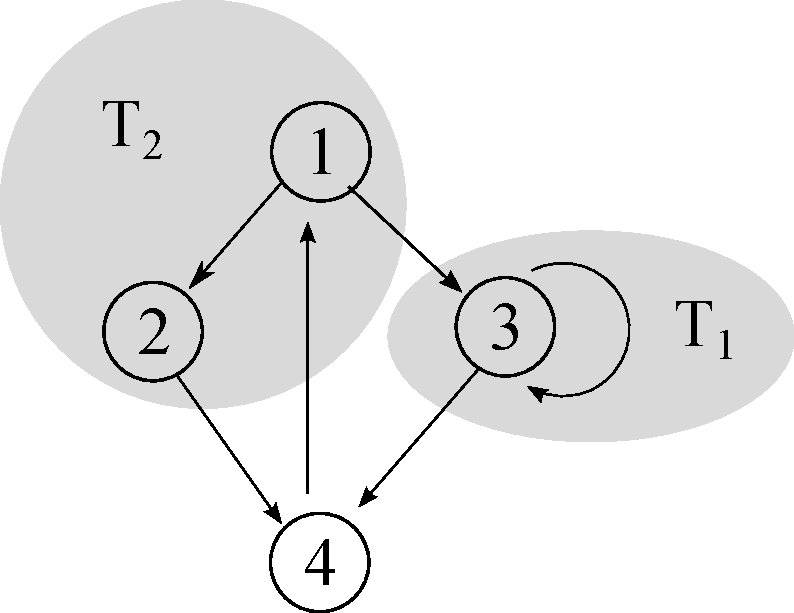
\includegraphics[width=5cm]{img/t1t2-1.pdf}
\end{center}
\caption{T$_{1}$-T$_{2}$-reduction}
\label{fig:t1t2-1}
\end{figure}

Our structural analysis is inspired by the
T$_{1}$-T$_{2}$-reduction~\cite{red_dragon}.  We say that a flow graph
is reducible if it can be reduced to a single node by the following
two transformations:

\begin{description}
  \item[T$_{1}$:] Remove an edge from a node to itself.

  \item[T$_{2}$:] Combine two nodes $m$ and $n$, where $m$ is the
    single predecessor of $n$, and $n$ is not the entry of the flow
    graph.
\end{description}

On \cref{fig:t1t2-1} is shown a small flow graph and highlights
instances where the two reductions could apply.  The overall idea is
to construct a flow graph of the Futhark program, reduce it to a single
point, and at each reduction step combine the information stored at
the nodes being combined.

Futhark always produces a reducible graph.  Each node corresponds to an
expression, with the successors of the node being its subexpressions.
This means that we can implement the reduction simply as a bottom-up
traversal of the Futhark syntax tree.

\begin{figure}[t]
\centering
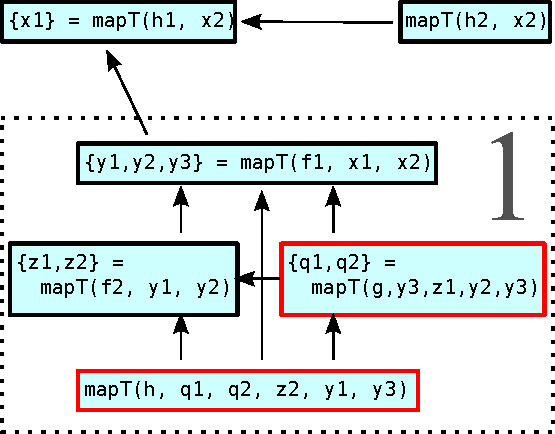
\includegraphics[width=35ex,valign=t]{img/fusion-1.pdf}\hspace{2ex}
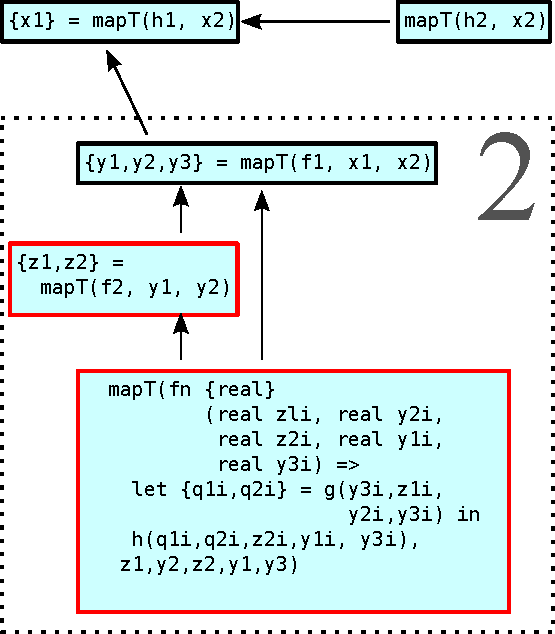
\includegraphics[width=35ex,valign=t]{img/fusion-2.pdf}

\hfill\vspace{2ex}\\

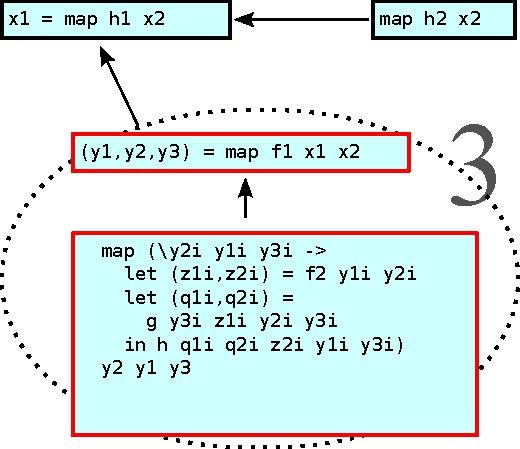
\includegraphics[width=35ex,valign=t]{img/fusion-3.pdf}\hspace{2ex}
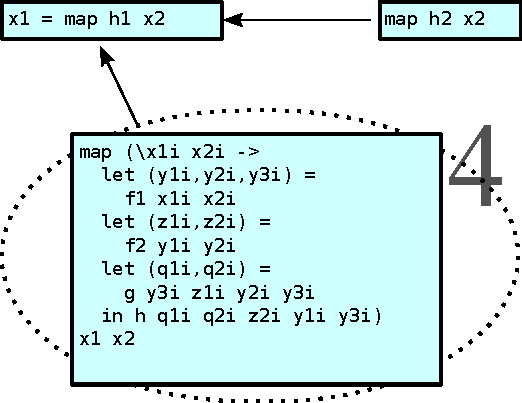
\includegraphics[width=35ex,valign=t]{img/fusion-4.pdf}
\caption{Fusion by T$_{2}$ transformation on the dependency graph}
\label{fig:fusion}
\end{figure}

Figure~\ref{fig:fusion} depicts the intuitive idea on which our fusion
transformation is based.  The top-left figure shows the dependency
graph of a simple program, where an arrow points from the consumer to
the producer.

The main point is that all SOACs that appear inside the box dashed box
can be fused without duplicating any computation, even if several of
the to-be-fused arrays are used in different SOACs.  For example,
\texttt{y1} is used to compute both \texttt{\{z1,z2\}} and
\texttt{\{q1,q2\}}\footnote{Note also that not all input arrays of a
  SOAC need be produced by the same SOAC.}.  This is accomplished by
means of $T_2$ reduction on the dependency graph:

The rightmost child, i.e., \texttt{mapT(g,..)}, of the root SOAC
(\texttt{mapT(f1,...)}) has only one incoming edge, hence it can be
fused.  This is achieved by:
\begin{enumerate}
\item Replacing in the root SOAC the child's
  output with the child's input arrays
\item Inserting a call to the
  child's function in the root's function, which computes the
  per-element output of the child,
\item Removing duplicate input arrays of the resulting SOAC.
\end{enumerate}
This operation is exactly what the fusion rules in
\cref{sec:fusion-rules} formalise.

The top-right part of \cref{fig:fusion} shows the (optimised) result
of the first fusion, where the copy statements have been eliminated by
copy propagation.  In the new graph, the leftmost child of the root,
i.e., the one computing \texttt{\{z1,z2\}}, has only one incoming edge
and can be fused.  The resulting graph, shown in the bottom-left
figure can be fused again resulting in the bottom-right graph of
\cref{fig:fusion}.  At this point no further $T_2$ reduction is
possible, because the SOAC computing \texttt{x1} has two incoming
edges.  This example demonstrates a key benefit of removing
\texttt{zip}/\texttt{unzip} and using the tupleless SOACs
representation: There are no intermediate nodes in the data-dependency
graph between fusable producer and consumer.

\subsection{Dataflow rules}

During reduction, we will track the following pieces of information.

\begin{description}
\item[$\soacs : Exp \rightarrow (Label \times Pat \times Exp) Set$.]
  The set of SOACs that appears in an expression, modelled as a
  mapping from a (unique) label to a pair of a SOAC expression and its
  output pattern.  We shall say $\soacs(e)$ to refer to this mapping,
  and $\soacs(e)[l]$ to refer to the SOAC with label $l$.  For
  example,
  \begin{align*}
  & \soacs(\texttt{let \{$a$,$b$,$c$\} = mapT($f$,$x$,$y$,$z$) in \{$a$,$b$,$c$\}}) =\\
  & \quad \{ (\ell, \texttt{\{$a$,$b$,$c$\}},\texttt{mapT($f$,$x$,$y$,$z$)}) \},
  \end{align*}
  where $\ell$ is a fresh label.  After the $\soacs$ set has been
  computed, we can use $\soacs(e_{b})$, where $e_{b}$ is the body of a
  function to refer to the set of all SOACS in that function.  Since
  the fusion transformation is strictly intraprocedural, this is
  sufficient for our needs.

  This mapping may not necessarily contain all SOACs that appear
  \textit{syntactically} in the program.  A core idea behind the
  fusion algorithm is that whenever we would add a SOAC to this
  mapping, we instead check whether it can be fused with the SOACs
  already present.

\item[$\infusible : Exp \rightarrow Name Set$.] The \textit{infusible
    set}, a set of variable names, is key to preventing unwanted
  fusion, as it indicates which SOACs should never be fused.  The
  infusible set prevents both undesired and invalid fusion, as
  outlined in sections \cref{sec:whentofuse,sec:invalidfusion}
  respectively.  Given an Futhark expression $e$, we shall say
  $\infusible(e)$ to refer to the infusible set produced by $e$.  For
  example:
  \begin{align*}
  \infusible(&\texttt{let x = mapT(f,a) in}\\
  &\texttt{let y = mapT(g,a) in \{x,y\}}) = \{a\},
  \end{align*}
  because $a$ is used twice, and hence fusing its producer into
  \texttt{f} and \texttt{g} would cause work duplication.  To simplify
  the example, $f$ and $g$ are ignored when computing the infusible
  set, although as we shall see below, this is not the case in
  practice.

\item[$\inputs : Exp \rightarrow Name \rightarrow Labels$.] A mapping from arrays to a set of the SOACs that use the array
  as input.  This is modelled as a set of pairs, each pair consisting
  of an array name and a SOAC name.  We shall refer to the mapping
  generated by a given expression $e$ as $\inputs(e)$.  For example,
  \[
  \inputs(\texttt{mapT($f$, $x$, $y$, $z$)}) = \{ (x, \{\ell\}), (y, \{\ell\}), (z, \{\ell\}) \},
  \]
  where $\ell$ is the label of the \texttt{mapT}-SOAC.

  We define an associative and commutative operation $\sqcup$ to
  combine multiset mappings by taking the union of values (in the case
  of $\inputs$, sets of labels, $s$) of corresponding keys (for
  $\inputs$, variable names, $v$), as follows.
  \begin{align*}
  &\{(v_{1},s_{1}),\ldots,(v_{n},s_{n})\} \sqcup \{(v_{n+1},s_{n+1}),\ldots,(v_{n+m},s_{n+m})\} =\\
  &\quad \{(v_{i}, \bigcup_{(v_{i},s_{j}),0 \leq j \leq n+m} s_{j})\},
  \end{align*}

  Intuitively, $x \sqcup y$ is a mapping that contains the union of
  the keys in $x$ and $y$, with the value for a key $v$ being the
  union of the values for $v$ in $x$ and $y$ (or just an untouched
  value, if $v$ was only present in one of the mappings).

  Similarly, we use $\sqcap$ to denote a similar mapping, except
  taking the intersection of values.
\begin{align*}
  &\{(v_{1},s_{1}),\ldots,(v_{n},s_{n})\} \sqcap \{(v_{n+1},s_{n+1}),\ldots,(v_{n+m},s_{n+m})\} =\\
  &\quad \{(v_{i}, \bigcap_{(v_{i},s_{j}),0 \leq j \leq n+m} s_{j})\},
  \end{align*}

\item[$\consumed : Exp \rightarrow Label \rightarrow Name Set$.] A
  mapping from the labels of SOACs in an expression, to a set of the
  names that are consumed on the path to that SOAC.  The purpose of
  this mapping is to ensure that we do not fuse in violation of the
  uniqueness rules.  For example, if
  \[
  consumed(e)[\ell] = \{\texttt{a}\}
  \]
  then we cannot fuse any producer taking \texttt{a} as input with the
  SOAC labelled $\ell$, as \texttt{a} is consumed on the execution
  path to $\ell$.
\end{description}

If more specific rules are not given, the data flows default to the
following.

\begin{align*}
  \infusible(e) &= \bigcup_{e'\in\childExps{e}} \infusible(e') \\
  \\
  \inputs(e) &= \bigsqcup_{e'\in\childExps{e}} e'\\
  \\
  \soacs(e) &= \bigcup_{e'\in\childExps{e}} \soacs(e') \\
  \\
  \consumed(e) &= \bigsqcup_{e'\in\childExps{e}} \consumed(e')
\end{align*}
Where $\childExps{e}$ are the \textit{immediate} children of $e$, e.g.
\[
\childExps{\texttt{if p(x) then t(y) else f(z)}} = \{\texttt{p(x)}, \texttt{t(y)}, \texttt{f(z)}\}.
\]

Now for specific rules, based on the shape of the given expression.

\begin{description}[style=nextline]
\item[Case $e \equiv v$ ($v$ is a variable)]

  This rule is only applied when $v$ is not an array input to a SOAC.
  This implies that the producer of $v$ cannot be fused, as its output
  $v$ is used here.
\begin{align*}
  & \infusible(e) = \{v\} \\
\end{align*}

\item[Case $e \equiv \texttt{$v$[$e_{1}$, \ldots, $e_{n}$]}$]

  If an element is retrieved from an array through indexing, we have
  no choice but to manifest that array, thus forcing us to avoid
  fusion due to our principle of avoiding duplication of computation.
  In many cases, for example if the array $v$ is the result of a
  \texttt{map} operation, it might be beneficial to replace the index
  operation by an inlined copy of the \texttt{map} function, and let
  the original \texttt{map} be fused.  Duplicating computation of a
  single element is likely acceptable, but not done in the general
  case by the current implementation, and it is hard to determine the
  optimal choice as long as Futhark does not yet have a well-defined
  cost model.  Nevertheless, \cref{sec:inlining-indexing} will
  describe how we inline particularly simple cases.
  \begin{align*}
  & \infusible(e) = \{v\} \cup \bigcup_{1\leq i \leq n}\infusible(e_{i}) \\
\end{align*}

\item[Case $e \equiv \texttt{if $e_{c}$ then $e_{t}$ else $e_{f}$}$]

  The \infusible{} of a conditional consists of whatever is in the
  \infusible{} sets of its branches, plus any SOAC outputs that may be
  used multiple times.  Note that an output can be used in both the
  true and the false branch, and it will still only have been
  considered to be used once, becase only one of the true and false
  branch will be executed, never both.

\begin{align*}
  & \inputs(e) =\\
  & \quad \{ (v,s')\ |\ (v,s) \in \inputs(e_{t}) \cup \inputs(e_{f}) \}\\
  & \quad\quad \text{Where $s'$ is the set of all SOAC consumers of $v$ in both $e_{t}$ and $e_{f}$.} \\
  \\
  & \infusible(e) =\\
  & \quad \infusible(e_{c}) \cup \infusible(e_{t}) \cup \infusible(e_{f})\\
  & \quad \cup (\inputs(e_{c}) \sqcap \inputs(e_{t}))\\
  & \quad \cup (\inputs(e_{c}) \sqcap \inputs(e_{f}))\\
\end{align*}

The reason for these rules can be illustrated by the following
examples.  In \cref{fig:fuse-across-if-ok}, it is clear that fusing
computation of \texttt{b} with both \texttt{map(g,b)} and
\texttt{map(h,b)} will not cause duplicated computation, as the two
consumers are on separate control-flow paths.  On the other hand, if
even one branch contains multiple uses, as in
\cref{fig:fuse-across-if-bad}, we should not fuse.  Additionally, if
both the conditional expression and a branch consumes the same array,
as on \cref{fig:fuse-across-if-bad-condition}, then we should also not
fuse.

\begin{figure}
\begin{center}
\begin{lstlisting}
let b = map(f, a) in
if p(x) then map(g,b)
        else map(h,b)
\end{lstlisting}
\end{center}
\caption{Fusion into branches acceptable}
\label{fig:fuse-across-if-ok}
\end{figure}

\begin{figure}
\begin{center}
\begin{lstlisting}
let b = map(f, a) in
if p(x) then concat(map(g,b),map(v,b))
        else map(h,b)
\end{lstlisting}
\end{center}
\caption{Duplicating computation in one branch}
\label{fig:fuse-across-if-bad}
\end{figure}

\begin{figure}
\begin{center}
\begin{lstlisting}
let b = map(f, a) in
if p(map(v,b)) then map(g,b)
               else map(h,b)
\end{lstlisting}
\end{center}
\caption{Duplicating computation in conditional}
\label{fig:fuse-across-if-bad-condition}
\end{figure}

\item[Case $e \equiv \texttt{loop ($p$ = $e_{1}$) = for $v$ < $e_{2}$ do $e_{3}$ in $e_{4}$}$]

  For loops, we add any arrays used as SOAC inputs in the loop body to
  the infusible set.  This is because fusing into the loop would
  duplicate computation by re-evaluating the function in the consumer
  for every iteration of the loop -- see \cref{fig:cannot-fuse-loop}
  for an example of this.  This is similar to how we ban fusing into
  SOAC-functions.

  Note that any use of an array for another purpose than as SOAC input
  results in that array name being present in $\infusible(e_{3})$
  already, thus banning fusion.
\begin{align*}
  & \infusible(e) =\\
  & \quad \infusible(e_{1}) \cup \infusible(e_{2}) \cup \infusible(e_{3}) \cup \infusible(e_{4}) \\
  & \quad \cup \{ v\ |\ (v,s) \in \inputs(e_{3}) \}
\end{align*}

\begin{figure}
\begin{center}
\begin{lstlisting}
let b = \emphh{map(f, a)} in
loop (v) = for i < n do
             let c = \emp{map(g, b)} in
             h(v,c) in
...
\end{lstlisting}
\end{center}
\caption{Fusing the \textit{producer} into the \textit{consumer} in the loop body would duplicate computation}
\label{fig:cannot-fuse-loop}
\end{figure}

\item[Case $e \equiv \texttt{let \{$\overline{vs}$\} = $soac$ in $e_{b}$}$]

  The big question here is whether $soac$ can be fused as producer
  with something in $\soacs(e_{b})$.  In the following, $\ell_{p}$ is
  a fresh name.  Let
  \[
  \zeta = \bigcup_{v \in vs} \inputs(e_{b},v)
  \]
  be the set of the labels of all SOACs that contain at least one of
  our outputs in their input set.

  For all $\ell^{c}_{i} \in \zeta$, we find the corresponding triple
  $(\ell^{c}_{i},vs^{c}_{i},soac^{c}_{i})$ in $\soacs(e_{b})$.  We can check
  whether fusion is possible by determining whether the following
  judgement is derivable.

\[
   \fusesto
    {vs}
    {soac}
    {soac^{c}_{i}}
    {soac^{r}_{i}}
\]

In total, the following four conditions must all be upheld before we
can fuse:

\begin{enumerate}
\item There must be at least one consumer $soac^{c}_{i}$ with which we
  can fuse.  Note that even if there are more than one, we do not end
  up duplicating computation, as they would belong to different
  branches.
\item For each consumer $soac^{c}_{i}$, we must be able to fuse and
  and get some $soac^{r}_{i}$.  If we could only fuse with some, we
  would be unable to remove the producer from the resulting program,
  thus duplicating computation.
\item None of $\overline{vs}$ are in the infusible set.  That is,
\[
\overline{vs} \cap \infusible(e_{b}) = \empty
\]
This rule also helps avoiding duplicate computation.
\item Fusion must not bring an array past a point where it is
  consumed.  Formally, we must have that,
\[
\consumed(e_{b})[\ell^{c}_{i}] \cap (\text{The array inputs of \(soac\)}) = \emptyset
\]
for all $\ell^{c}_{i}$.  Violating this rule would create an invalid
program.
\end{enumerate}

\begin{description}
\item[If the four conditions are true:]

  In this case, we are fusing $soac$ with several SOACs
  $soac^{c}_{i}$, each with a corresponding label $\ell^{c}_{i}$, and
  fused as $soac^{r}_{i}$.  In the following, let $e_{f}$ be the body
  of the function in $soac$.

\begin{align*}
  & \soacs(e) =\\
  & \quad (\soacs(e_{b}) \backslash \zeta)\\
  & \quad \cup \soacs(e_{f})\\
  & \quad \cup \{ (\ell^{c}_{i}, (vs, soac^{r}_{i}))\ |\ \textrm{for each $soac^{c}_{i}$} \}\\
  \\
  & \inputs(e) =\\
  & \quad (\textrm{$\inputs(e_{b})$ with all mappings to each $\ell^{c}_{i}$ removed}) \\
  & \quad \sqcup \{ (v,\ell^{c}_{i})\ |\ \textrm{for all array inputs $v$ in each $soac^{c}_{i}$} \}\\
  \\
  & \infusible(e) =\\
  & \quad \infusible(e_{b})\\
  & \quad \cup \{ v\ |\ (v,s) \in \inputs(e_{f}) \} \\
\end{align*}

\item[If they are not:]

  We cannot fuse with $soac$ as a producer, and we must add it as a
  kernel by itself.  It may be fused as the consumer at some later
  stage of the algorithm, however.  To the $\infusible$ set, we first
  add every array variable used as a SOAC input in the body of $soac$.
  We also also insert every array variable used both as input to
  $soac$, but also to some SOAC in $e_{b}$.  The rationale is that
  fusing whichever SOAC (if any) outputs this variable would duplicate
  computation, as we have at least two consumers.

\begin{align*}
  & \infusible(e) =\\
  & \quad \infusible(e_{b})\\
  & \quad \cup \{ v\ |\ (v,s) \in \inputs(e_{f}) \} \\
  & \quad \cup \{ v\ |\ \textrm{$v$ is used as input to $soac$ but is also in $\inputs(e_{b})$} \}\\
  \\
  & \inputs(e) =\\
  & \quad \inputs(e_{b})\\
  & \quad \sqcup \inputs(e_{f})\\
  & \quad \sqcup \{(e_{1},\{\ell_{p}\}), \ldots, (e_{n},\{\ell_{p}\})\}\\
  \\
  & \soacs(e) = \soacs(e_{b}) \cup \{(\ell_{p}, (vs, soac))\} \\
  &
\end{align*}
\end{description}

\item[Case $e \equiv \texttt{let $v_{1}$ = $v_{2}$ with [$e_{1}$,\ldots,$e_{n}$] <- $e_{v}$ in $e_b$}$]

  For any SOAC $\ell$ in the body $e_{b}$, we note that the aliases of
  $v_{2}$ are consumed on the path to $\ell$.

\begin{align*}
  & \consumed(e) =\\
  & \quad \{ (\ell, \aliases{v_{2}} \cup \consumed(e_{b})[\ell])\ |\ (\ell,p_{\ell},e_{\ell}) \in \consumed(e_{b}) \}
\end{align*}

\end{description}

%%% Local Variables:
%%% mode: latex
%%% TeX-master: "thesis"
%%% End:
